\chapter{How to update your ToM+ firmware}

\section{Requirements before updating}

ToM+ is constantly evolving, since quite every day I receive suggestions to improve
some features or even adding some cool ones. I'm trying to consider all pieces of
advice from each owner and these tips and ideas will result in firmware updates.
While testing the device on drive, if you notice bugs or weird stuff please report
them to me and they will result in firmware patches. As I said at the beginning,
ToM+ is constantly improving, so stay tuned\ldots

\subsection{Why should I update?}

Well, new update means new features and bug fixes, so why should you keep the old
firmware version when you can easily install the latest stable one? So, there's no
reason to keep your ToM+ outdated, since upgrading its software is \textbf{free forever}
and gives you a lot of satisfaction and fun while trying out new features. In the end, I personally
advice you to keep your ToM+ updated and safer.\\

Anyway all older firmware versions are still available on the Twizy forum in ToM section
(\url{https://www.twizy-forum.de/twiz-o-meter}) under \textit{“[Twiz o'meter] Update to
firmware x.x”} topics. In fact, ToM+ allows downgrades too, if needed.

\subsection{What do I need to update?}

In the next sections will be discussed an alternative way to update, much more
time consuming compared to the OTA method already discussed in Section~\ref{sec:web_ota_update}.
I personally \textbf{suggest the OTA method}, because it's safer and easier to do if you're not
really into IT and embedded systems.\\

If you're still convinced to upgrade ToM+ firmware with the second method, there are
a couple of things you will need in order to complete the update successfully. First
of all, you will need a computer and both desktops or laptops are great for this work.

Later we will see how to connect ToM+ to our computer in order to transfer the new
upgrade files on it. The second thing you must get is a micro USB cable, which is
the same that is usually used in rechargeable device and older smartphones. You will
also need a microSD card with a storage capacity between 8 and 32 GB. Examples
are shown in the photos down below. And of course you will need your ToM+!

\begin{figure}[H]
    \centering
    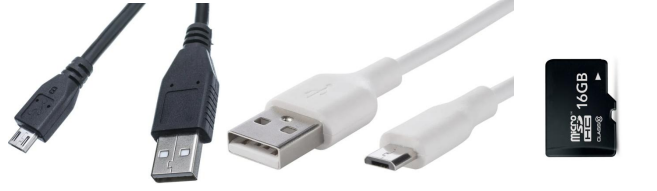
\includegraphics[width=0.8\textwidth]{figures/cables_sd_update.png}
    \caption{microUSB cables and example microSD card.}
\end{figure}


\subsection{How do the update files look like?}
\label{sec:update_files}

Before you update the firmware, you obviously need to download from the Twizy forum
(again \url{https://www.twizy-forum.de/twiz-o-meter}) the desired version update ZIP.
You will probably need to register to the forum to see and download firmware files and
images. It's a really cool and active community, so I suggest to become a member anyway.
After extracting the files in the folder, this is what you should get:

\begin{figure}[H]
    \centering
    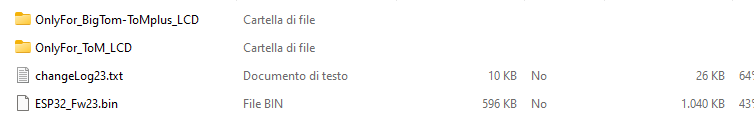
\includegraphics[width=1\textwidth]{figures/firmware_release_folder.png}
    \caption{Firmware release folder files list.}
\end{figure}

First of all, we notice a text file with the \textit{changeLog23.txt}, used to track
the added features and bug fixed in the latest firmware release. Read it if you are
curious to know what's new or if you need additional help with the update procedure.\\

Next, there are two folders containing the \textbf{LCD display firmware} update in a \textit{.tft}
format. \textbf{Choose the version} made for your device: first folder if you got a ToM+ or a
BigToM (that means bigger display) or the other one if you have a traditional ToM or
you're willing to update the Twin ToM (smaller screen). This is a crucial
step, otherwise new icons and graphics won't fit your display size.\\

The last one is the \textit{ESP32\textunderscore Fw23.bin} binary file for the \textbf{black box update}.
Make sure to have all of these files, because you will need them in the next steps.

\subsection{What should I know before update?}

Now let's prepare our ToM+ to be updated by \textbf{toggling OFF the switch} on the
black box. Make sure to switch it off (\textit{i.e. 0 symbol on the switch}) or you
will surely cause serious problems to ToM+.

So, if your Twizy is still powered on with the key in, simply switch it completely off
and remove the ignition key. After this easy steps, you are ready to get into the update
procedure, but remember to strictly follow the steps discussed in the guide. Don't
proceed by intuition, otherwise you will risk to permanently brick your device.\\

The upgrading process is quite easy and you will need to update both the LCD firmware
and the black box one, in this specific order. We will see how in the next section.



\section{Updating LCD firmware}

The LCD display is one of the essential parts of ToM+ as it was discussed in the first
two chapters and for this reason it will need to be updated as well. New firmware
means new icons and different layouts and, in order to upload the new ones onto it,
it's crucial to use a small \textbf{microSD card} to accomplish this task. ToM+ SD
card slot is under the display so you may need to temporarily remove it from your
glove box so that you can better work on it, or simply tilt it backwards and you 
will see the hole.

\subsection{Preparing the microSD card}

Unfortunately, not all microSD cards are working with the display, especially newer
ones made for cameras, but for now I have tried class 10 HC 8 to 32 GB ones and they
seem to work well. But feel free to try with your own memory card and see if it works.\\

Now that we've chosen a microSD card, that must have a storage capacity \textbf{between 8
and 32 GB}, we need to copy the LCD firmware on it. Before copying the file on
it, we must make sure that there aren't any other files or the upgrade won't work.

So, move any files to your computer and format the microSD card in a \textbf{FAT32 format}
as I did in the screenshot here. To achieve that right, click on the card icon in your file
explorer and select the \textbf{“Format”} option from the dropdown menu.

\begin{figure}[H]
    \centering
    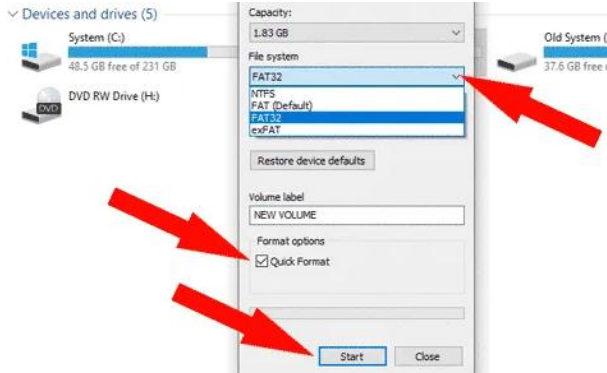
\includegraphics[width=0.7\textwidth]{figures/forma_sd_steps.png}
    \caption{How to FAT32 format microSD steps.}
\end{figure}

As it's shown in the picture, select \textbf{FAT32} file system, then check the 
\textbf{“Quick Format”} option and press the \textbf{“Start”} button to begin the 
process. Wait until it's finished and then copy the \textit{.tft} file attached in
the firmware release you want to install, contained in the update ZIP folder.


\subsection{Inserting the microSD card}

Now, we are ready to put the microSD card in the LCD display slot. It may help 
using some snipe nose pliers to carefully insert the microSD card. This should
ensure you would center the internal SD card slot.\\

\textbf{REMEMBER!} The microSD card fits in the slot only in one way, with the contacts
side pointing to the screen surface, as shown in the image. If it doesn't, don't force it!
Try turning it to the other side.

Now that the microSD card is inserted in the internal slot, slowly push it into the 
box until your hear a “click” sound. This will mean that you can safely remove the 
pliers without losing the card inside the box.

\begin{figure}[H]
    \centering
    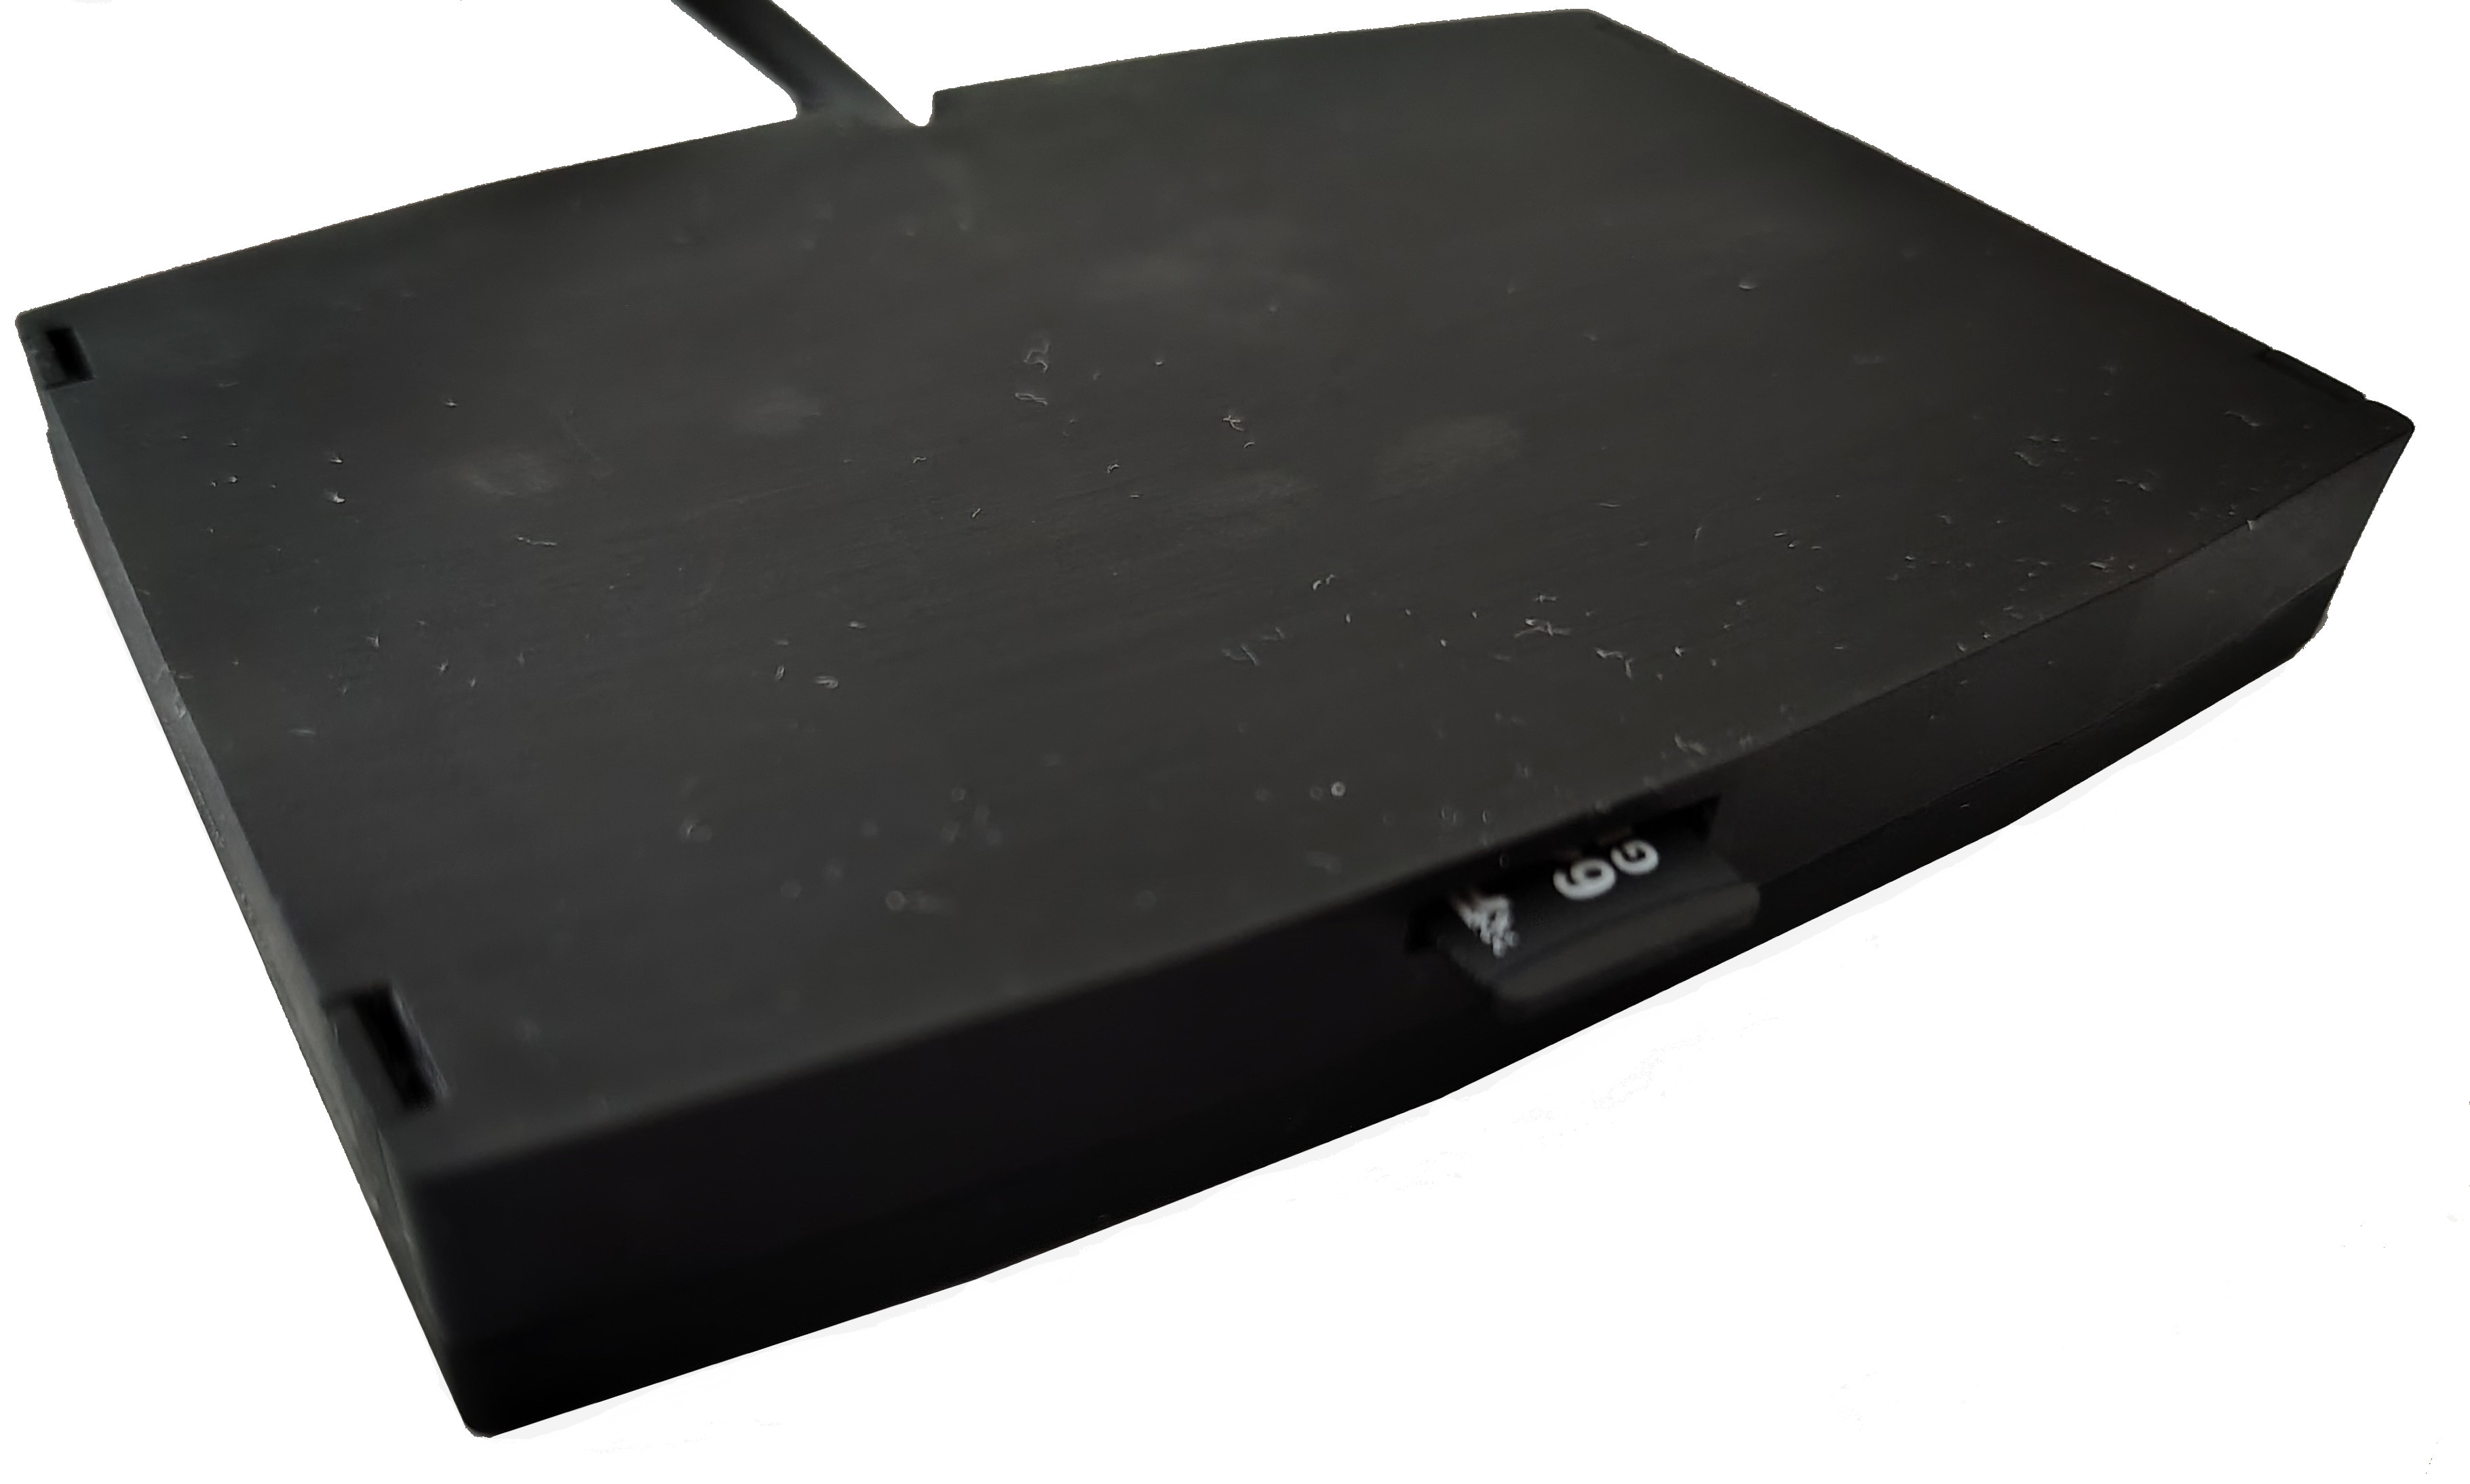
\includegraphics[width=0.6\textwidth]{figures/sd_insert.jpg}
    \caption{Insert the microSD in the display hole.}
\end{figure}


\subsection{The updating workflow}

Once the microSD is in, we can carry on with the updating workflow. Now, let's get
back to our Twizy and plug the display back to the black box. Then, power on the
display using the switch on the black box (\textit{i.e. 1 symbol on the switch}) and,
only after that, power on your Twizy using the ignition key.

Wait for the LCD display to start the updating process until you see the progress
percentage as shown in the figure below (both for the ToM+ and ToM display). 
The microSD copying process will usually take up to a minute and a half.

\begin{figure}[ht]
    \centering

    \begin{subfigure}[t]{0.48\textwidth}
        \centering
        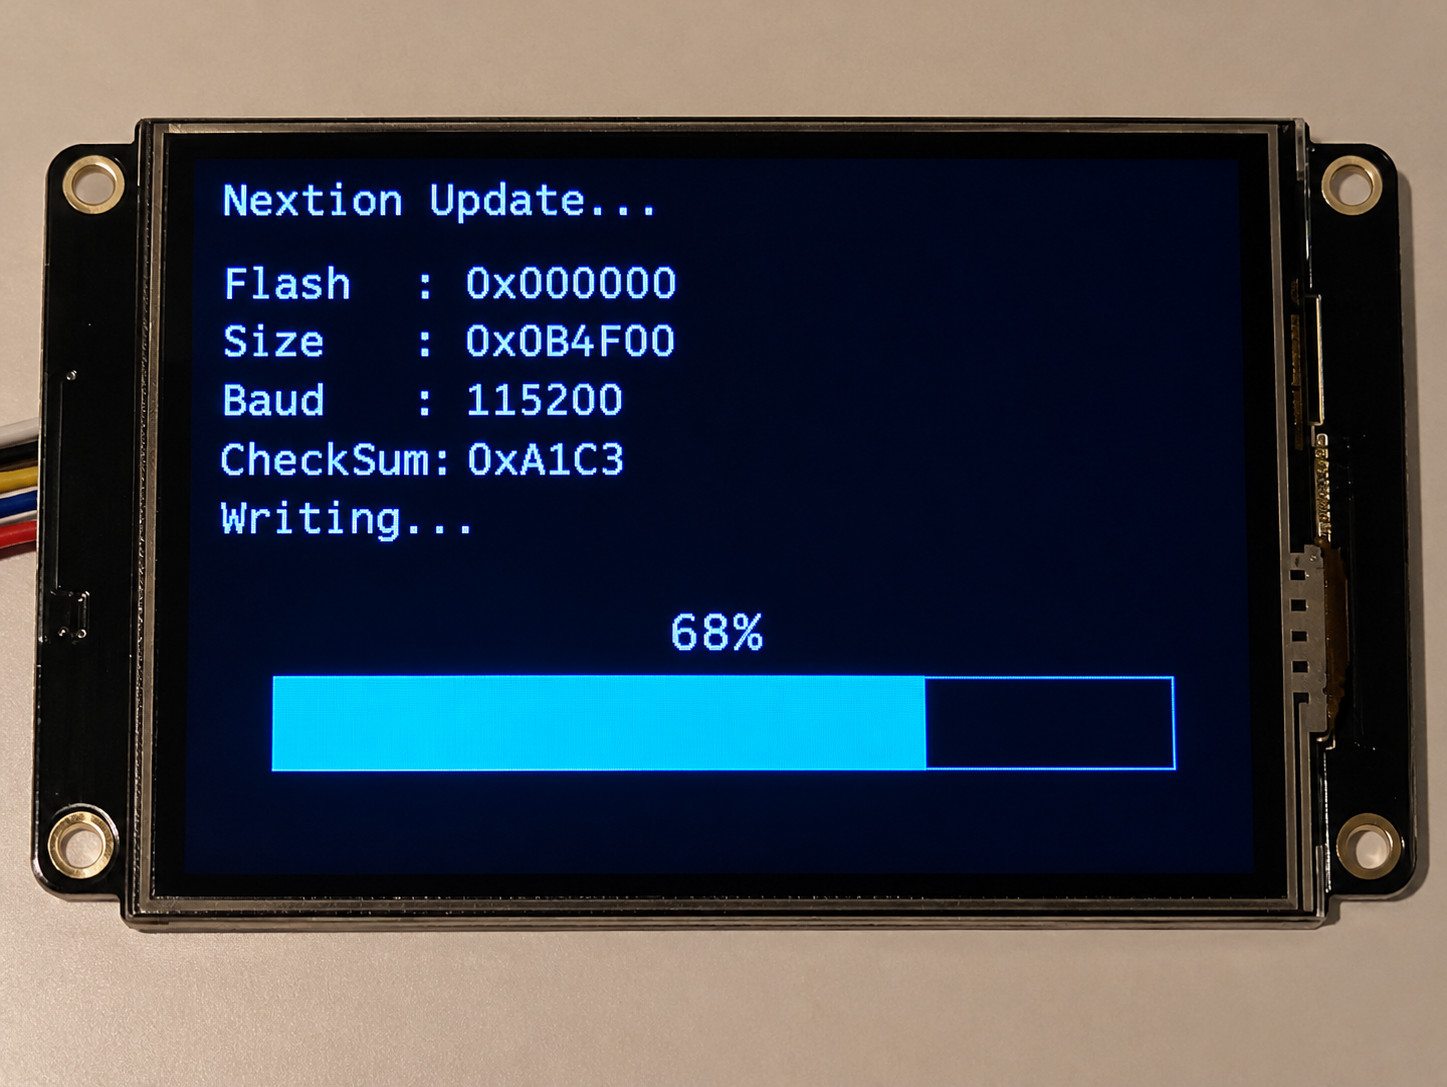
\includegraphics[width=\linewidth]{figures/update_screen_lcd.jpg}
        \caption{ToM+ display update.}
    \end{subfigure}
    \hfill
    \begin{subfigure}[t]{0.48\textwidth}
        \centering
        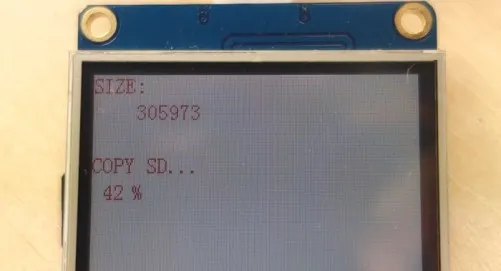
\includegraphics[width=\linewidth]{figures/copy-sd-card-nextion.png}
        \caption{ToM display update.}
    \end{subfigure}
\end{figure}

Once the updating of the LCD firmware is completed successfully you will see this
screen, saying that the \textbf{“Update Succeeded!”}. After update, \textbf{DON'T}
power on with the microSD inserted! Now, we can power off the car and the switch OFF
ToM+ again using the switch on the black box.

Then, remove the microSD card while the whole system is powered off and the LCD 
update is complete. \textbf{REMEMBER!} If you remove the card with ToM+ powered on
you will permanently brick the device! After that, without changing the state of the
overall system let's proceed with the black box update, as shown in the next section.



\section{Updating black box firmware (Windows)}

The black box is the second essential component of ToM+ and it's the brain of the
whole system. If we update the display only, then the black box won't know what
those new icons are intended for and this will cause mismatches in the communication.

So it's crucial to mount the new firmware on the motherboard of ToM+ as well. To do
that, we won't need the microSD card anymore, but we will use the microUSB cable
we prepared before and the computer. In fact, we will flash the firmware directly on
the ESP32 board to mount the new software.


\subsection{Preparing the computer}

Before plugging the cable in the computer, we need to install some programs to let it
work properly. The \textbf{ESP32 board} needs some drivers to be recognized by the
operative system, so we will download them directly from the official website.

From the download page of the \href{https://www.silabs.com/software-and-tools/usb-to-uart-bridge-vcp-drivers?tab=downloads}{Silicon Lab website},
we need to choose our operative system version, as we can see in the screenshot I've taken down here.

\begin{figure}[H]
    \centering
    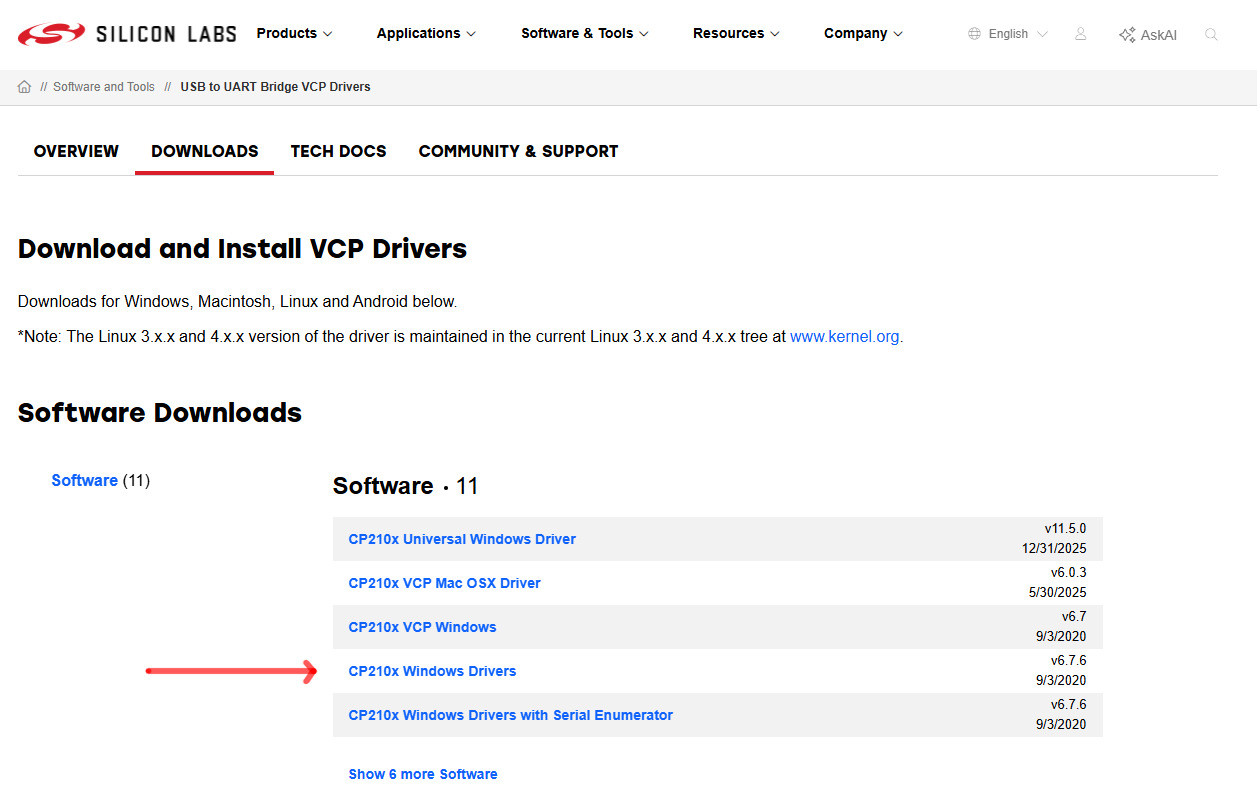
\includegraphics[width=1\textwidth]{figures/driver_download.png}
    \caption{Driver dowload page on Silicon Lab.}
\end{figure}

Since this section of the guide is specific to any Windows operative system we will
download the \textit{“CP210x Windows Drivers”} package pressing on the link pointed
in yellow in the image above.

The downloaded file will be a ZIP folder, usually called \textit{“CP210x\textunderscore Windows\textunderscore Drivers.zip”}
in which you can find a couple of folders and some files. In the screenshot below
are listed all the usual files contained in the ZIP folder.

\begin{figure}[H]
    \centering
    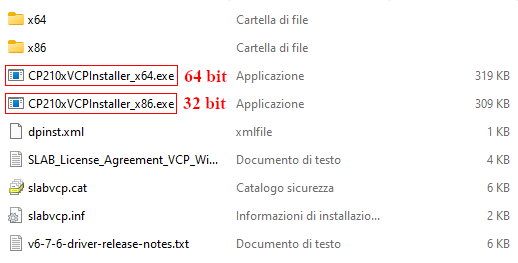
\includegraphics[width=0.7\textwidth]{figures/driver_folder.png}
    \caption{Contents of driver ZIP folder.}
\end{figure}

Extract all the files in a dummy folder in your Desktop. Now, it's important to
choose the right \textit{“.exe”} file to run in order to install the drivers. If your
operating system is 64 bit (for most computers) you will run \textit{CP210xVCPInstaller\textunderscore x64.exe}
file, otherwise the second \textit{“.exe”} file is the properly one, as show in the image.

Make sure to run the executable file with admin permission by right clicking on it and
selecting \textbf{“Run as Administrator”} option. If prompted allow the program to perform
admin operations on your computer, or the driver installation process won't start.

\begin{figure}[ht]
    \centering

    \begin{subfigure}[t]{0.48\textwidth}
        \centering
        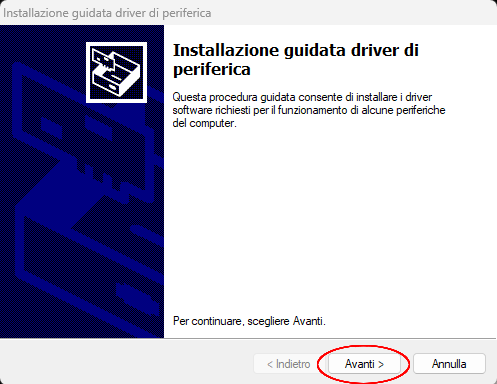
\includegraphics[width=\linewidth]{figures/wizard_step1.png}
        \caption{First step: Press “Next”.}
    \end{subfigure}
    \hfill
    \begin{subfigure}[t]{0.48\textwidth}
        \centering
        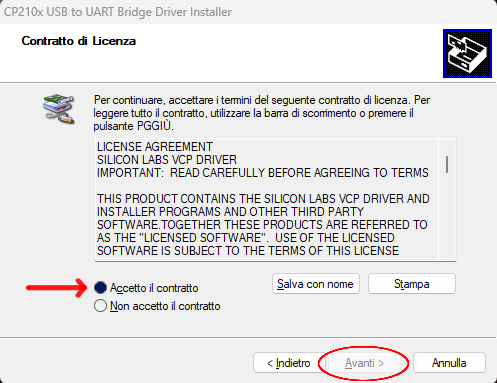
\includegraphics[width=\linewidth]{figures/wizard_step2.png}
        \caption{Second step: “Accept” and “Next”.}
    \end{subfigure}
\end{figure}

Once the installer starts you will see a window like the one shown on the left. This is a
wizard tool to install the drivers you will need to recognize the black box from your
computer. Now let's press the \textbf{“Next”} button as shown here to start the whole process.\\

The next window you will probably see is this one shown on the right. Here
you must accept the license by checking the first button \textbf{“Accept the license”}. Then,
you can press the \textbf{“Next”} button as shown here and start the copy of the drivers
in the right system folder: wait for the copy to finish.

When the copy is done, the installation of CP210X drivers is complete and you can
safely plug in the black box into your computer. Now press the \textbf{“Finish”}
button to close the window.\\

Before doing anything make sure that the switch on ToM+ black box is powered
OFF (\textit{i.e. 0 symbol on the switch}). The Twizy must be powered off as well
because, if you try plugging the cable in your PC while ToM+ is still powered by the
car, you will mix power supplies (5V and 12V) and ToM+ will definitely die.

\begin{figure}[H]
    \centering
    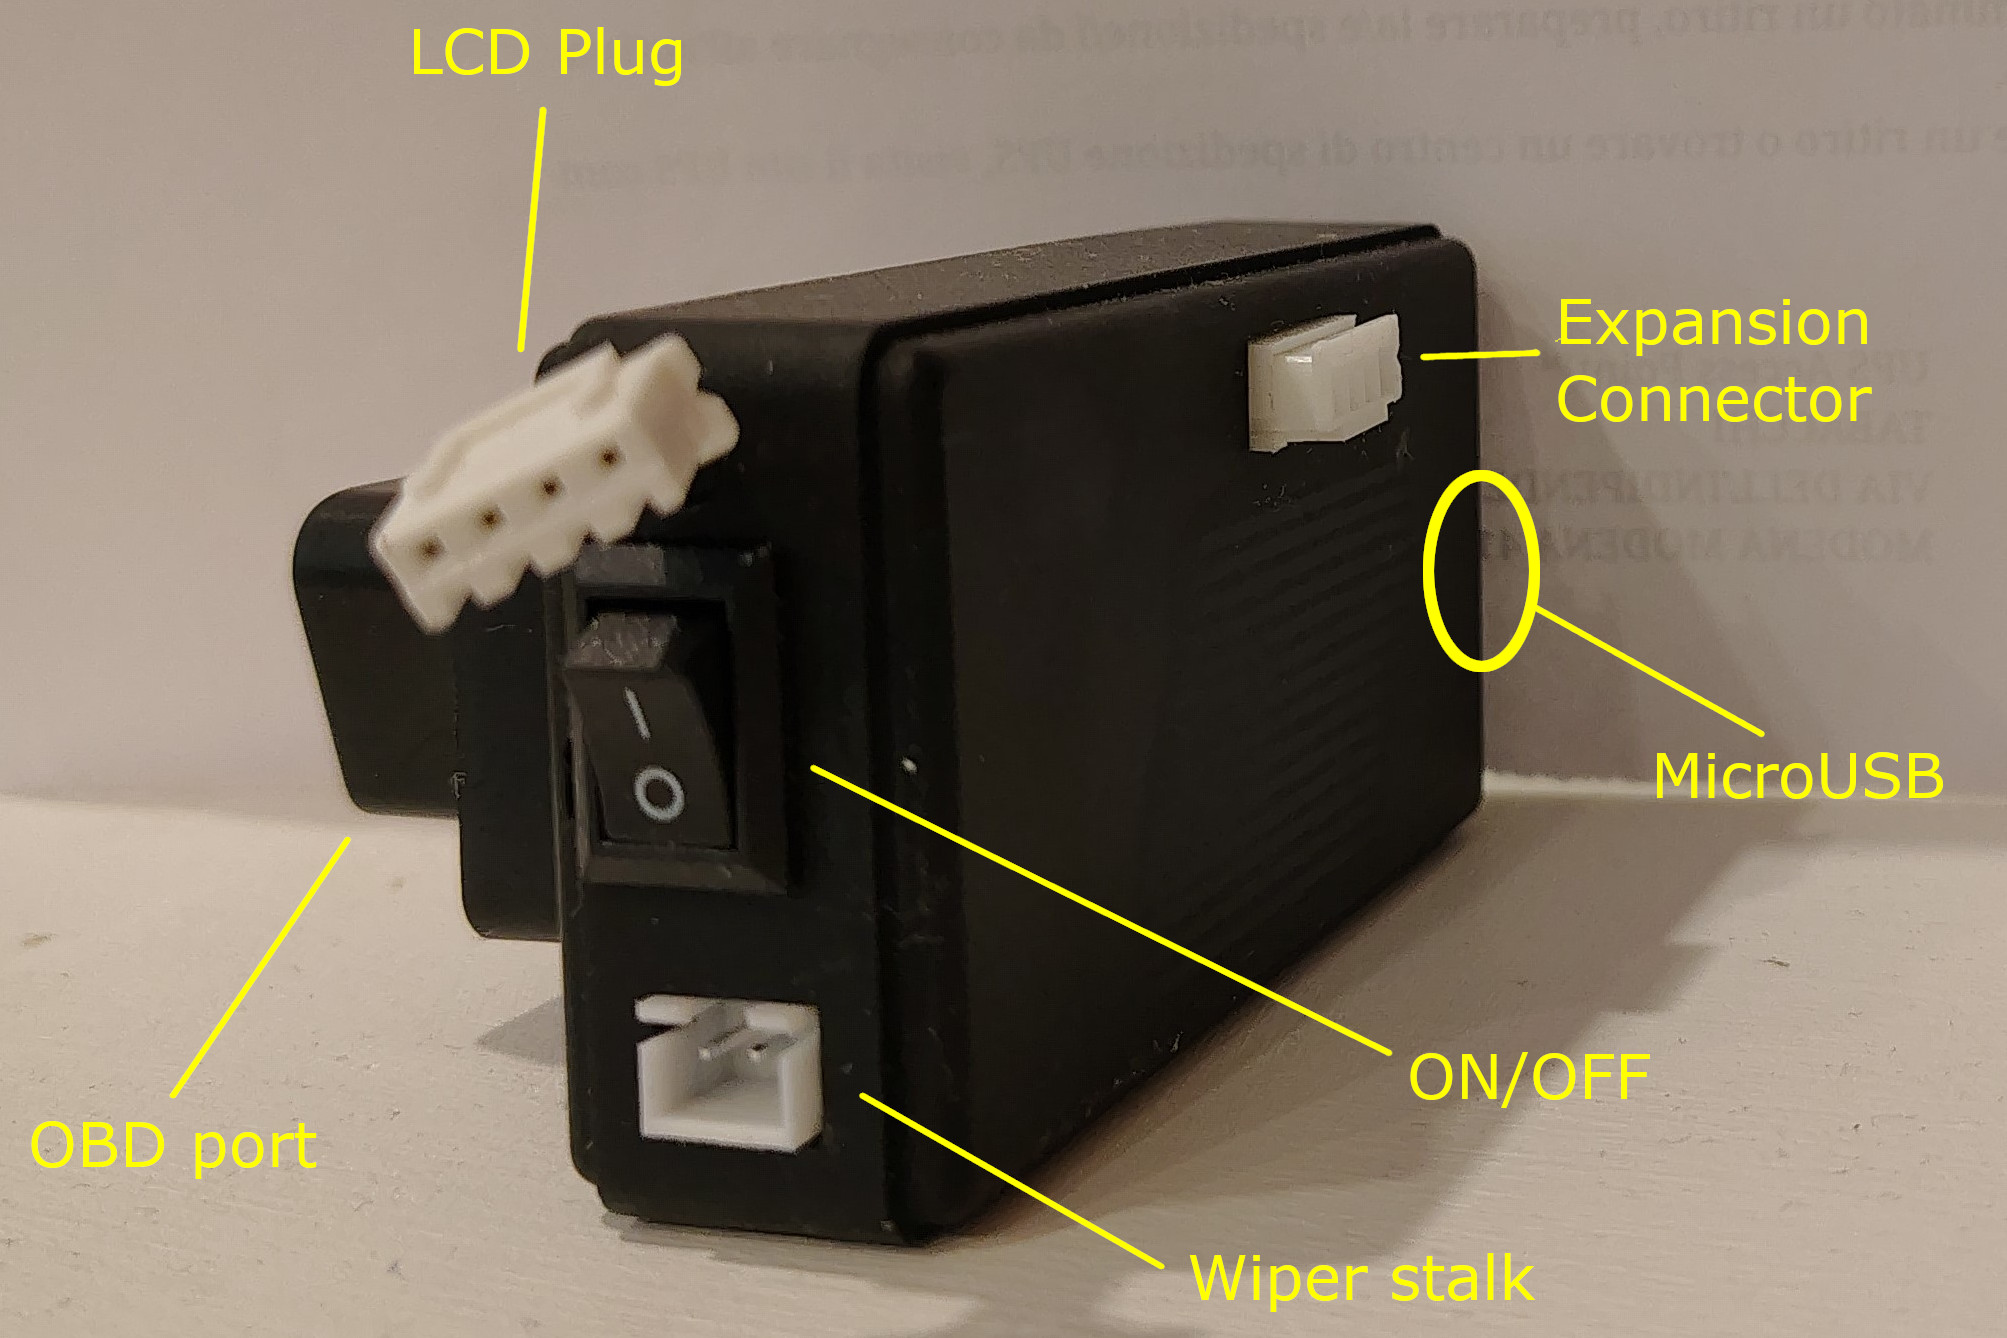
\includegraphics[width=0.6\textwidth]{figures/black_box.jpg}
    \caption{The black box components.} \label{fig:black_box_labels}
\end{figure}

The black box has a small microUSB connector on the rear side, as
you can see in the image above. So, connect the microUSB cable side and to the black box.
After that, connect the USB side of the cable to a free USB port on your computer.

\textbf{REMEMBER!} Both sides of the cable fits only in one way in the corresponding
plugs, so don't force them or you will risk to brake the ToM+ port or your computer one.
Try turning it to the other side and check if it works that way.\\

Now the computer should recognize the black box ESP32 board, if you installed the
drivers properly. To check if it's so, search for the \textbf{“Device Manager”} app
on your PC and run it.

Now you should have opened a window that looks like the one shown in the figure
down below. Find the \textbf{“Ports”} row with a connector icon and double click it, opening
the list of all of your serial devices. As I did in the screenshot look for \textit{“Silicon Labs
CP210x to UART Bridge (COMx)”} and then note down the COM number, that is
\textbf{COM8} in the example. This number will be useful in the next step to tell the PC
where to upload the new firmware version. Let's continue this process\ldots

\begin{figure}[H]
    \centering
    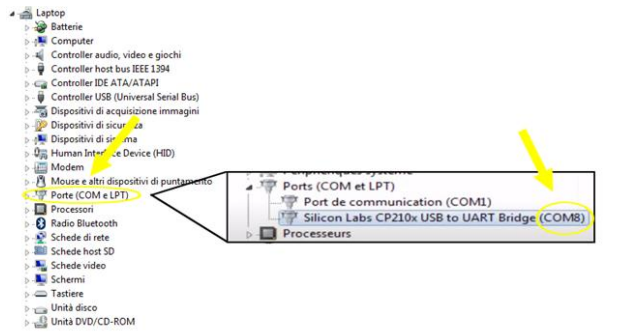
\includegraphics[width=0.8\textwidth]{figures/device_manager.png}
    \caption{Device manager UART serial port (COM8).}
\end{figure}

Visit the \href{https://www.espressif.com/en/support/download/other-tools}{ESP32 official website}
to download a tool that we will need to flash the firmware on our black box board.
Look for \textbf{“Flash Download Tools”} and press the button as shown in the image.
Then, search in the page for the \textit{“Flash Download Tools”} with the save icon and press it.

It will download a ZIP folder called \textit{“flash\textunderscore download\textunderscore tool\textunderscore x.x.x.zip”},
where the “x” symbols will be replaced by the version name, which is \textbf{V3.9.11} in this example.
Opening the downloaded ZIP folder, you will notice that there is another folder in it.
Extract that one on your Destktop or wherever you want and open it. The files
contained in it would usually be the ones listed in the screenshot below.

\begin{figure}[H]
    \centering
    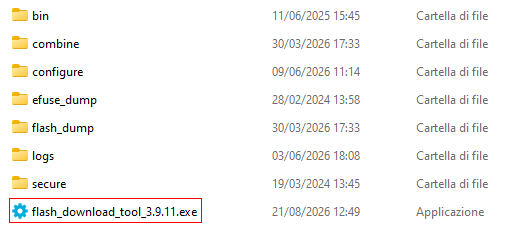
\includegraphics[width=0.7\textwidth]{figures/esptool_folder.png}
    \caption{Contents of Flash Tools ZIP folder.}
\end{figure}

Select the \textit{“flash\textunderscore download\textunderscore tool\textunderscore 3.9.11.exe”}
or whatever version you downloaded and run it with admin permissions, by right clicking
on the file and selecting \textbf{“Run as Administrator”} option.
If prompted, allow the executable file to perform operations on your computer.\\

Once the program is started, you should see a terminal window opening, that is going
to lunch in some seconds the user interface. It should look like as the first one
shown in the example here. You need to change the \textbf{“ChypType”} to \textit{“ESP32”}
as it's shown in the second step down below. Leave the rest as it is and press \textbf{“OK”} button.

\begin{figure}[H]
    \centering
    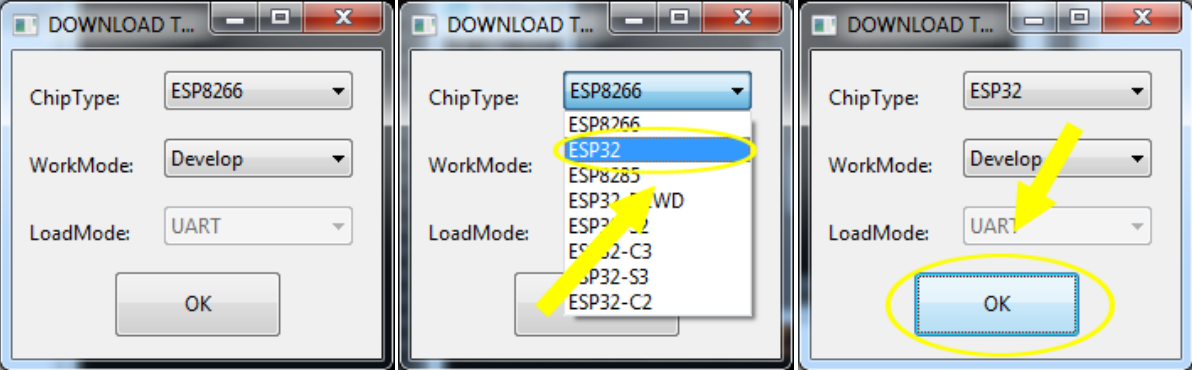
\includegraphics[width=0.85\textwidth]{figures/launching_flashtool.png}
    \caption{Select ESP32 motherboard in the choice box.}
\end{figure}


\subsection{The updating workflow}

As soon as you press the \textbf{“OK”} button a \textit{“ESP32 DOWNLOAD TOOL”} window will
open. Now, extract the binary file (\textit{.bin} extension) attached in the ToM+
firmware release ZIP as we discussed in Section~\ref{sec:update_files}.

Then, press the \textbf{“\ldots”} button shown in the first image and select the path of the \textit{“.bin”}
file. Once you did that, press the \textbf{“Open”} button and you will see a green record in the
first line containing the path you've just confirmed.

Proceed by \textbf{flagging the check box} next to the first line, choosing the firmware you
want to upload. Then, type in the text box shown in the second picture this sequence
of characters: \textbf{0x10000} (with four zeros). This represents the starting memory
address where the firmware files will be stored.

Now, it comes the last step of the configuration: select the COM number
using the list box in the bottom right corner. Make sure to select the right COM,
which is the one we previously note down from the \textbf{Device Manager} page.

\begin{figure}[H]
    \centering
    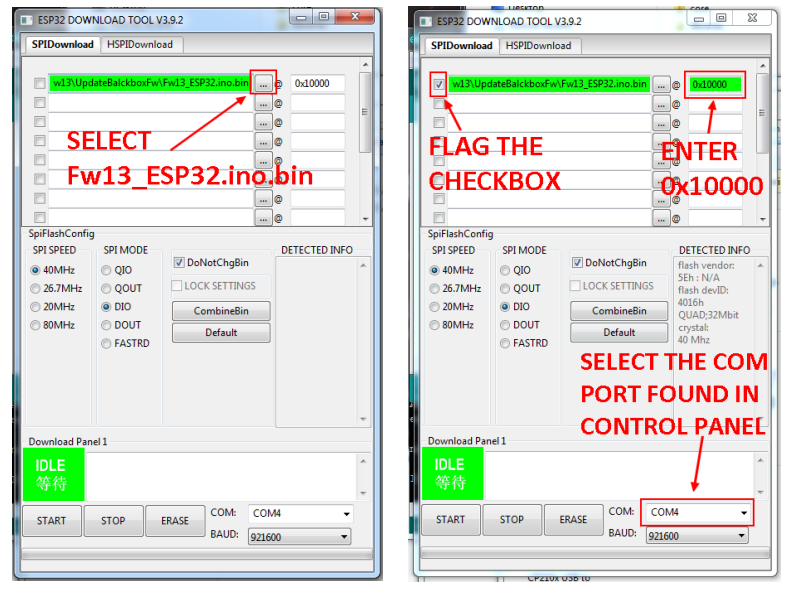
\includegraphics[width=1\textwidth]{figures/flashtool_page.png}
    \caption{ESP32 Download Tool configuration steps.}
\end{figure}

Now let's start the update pressing the \textbf{“START”} button as shown in the first picture.
A green progress bar will appear in the bottom of the window and the whole process
should usually take a couple of minutes.

Once the upload is completed, you will see a \textbf{“FINISH”} message in the green
box at the bottom left corner, as shown in the image.
As an additional confirm, the progress bar will be full and now the update is done.

\begin{figure}[H]
    \centering
    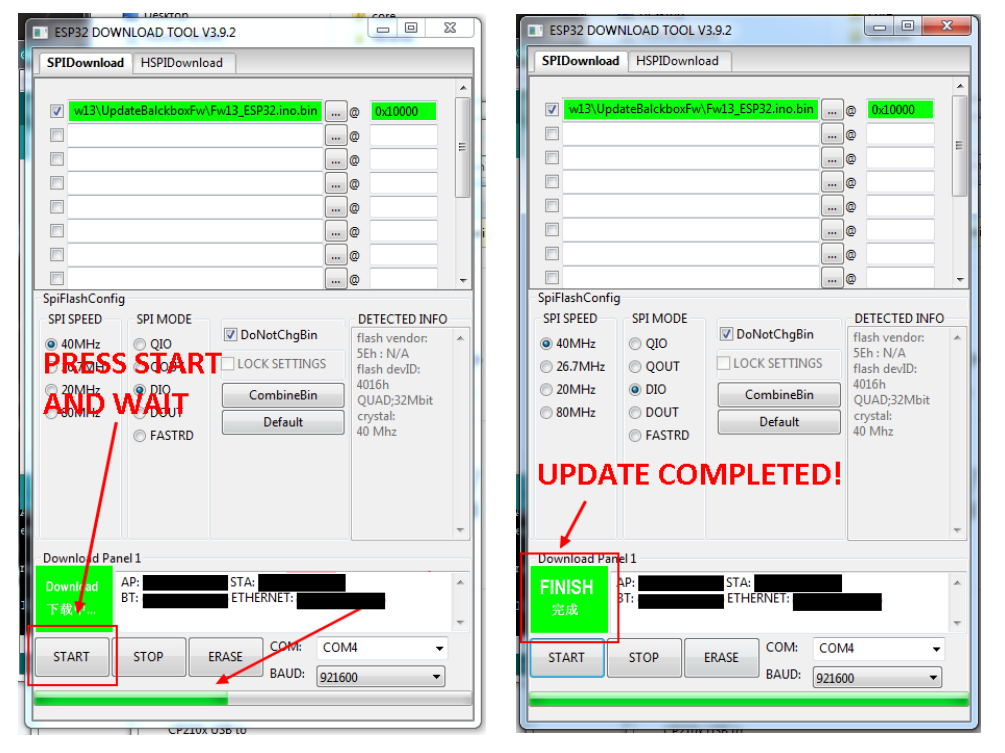
\includegraphics[width=1\textwidth]{figures/flashtool_page2.png}
    \caption{ESP32 Download Tool finalizing update.}
\end{figure}

Now close this window and then you can safely unplug the cable from both your PC
and ToM+. Only after this actions, you can restore the normal power supply of ToM+,
moving the switch to the 1 state and powering on your Twizy using the ignition key.

To restore your previous configurations, enter in the ToM+ settings page by pressing
the three dots in the top right corner and then press the exit button without doing
anything. Doing that way you will update the data structure saved in black box
memory and your configurations are back too.\\

\textbf{Congratulations!} You've finished the whole updating process, now enjoy the new firmware
and remember to report any bugs or problems to me through private messages, attaching 
an image perhaps.

\clearpage

\section{Updating the black box (Unix)}

The black box is the second essential component of ToM+ and it's the brain of the
whole system. If we update the display only, then the black box won't know what
those new icons are intended for and this will cause mismatches in the communication.

So it's crucial to mount the new firmware on the motherboard of ToM+ as well. To do
that, we won't need the microSD card anymore, but we will use the microUSB cable
we prepared before and the computer. In fact, we will flash the firmware directly on
the ESP32 board to mount the new software.

Before doing anything, turn OFF ToM+ black box switch (\textit{i.e. 0 symbol on it})
and power off your Twizy as well. It's an important step to strictly follow to avoid
damages to the device.

\subsection{Preparing the computer}

Download the ToM+ firmware update folder attached to the firmware release post.
Now, extract the binary file (\textit{.bin} extension) attached in the ToM+
firmware release ZIP as we discussed in Section~\ref{sec:update_files}.
The file in it is usually called \textit{“FwXX\textunderscore ESP32\textunderscore rel.bin”},
where the \textit{“XX”} symbol will be replaced by the version number, for instance \textit{“23”}.\\

\textbf{Disclaimer:} \textit{this black box process was tested using Ubuntu 20.04
(hope it will work with other Unix distribution too). Do not plug the black box until
explicitly told to do so}.\\

Now we need to install the esptool package, to flash the new firmware onto the black
box. Do this, either with the package manager UI provided by your Unix distribution, or
with the appropriate command in a terminal. For instance, \textit{“sudo apt-get esptool”},
as shown in the image. If prompted, type in the password of the sudo user, then press ENTER and wait.

\begin{figure}[H]
    \centering
    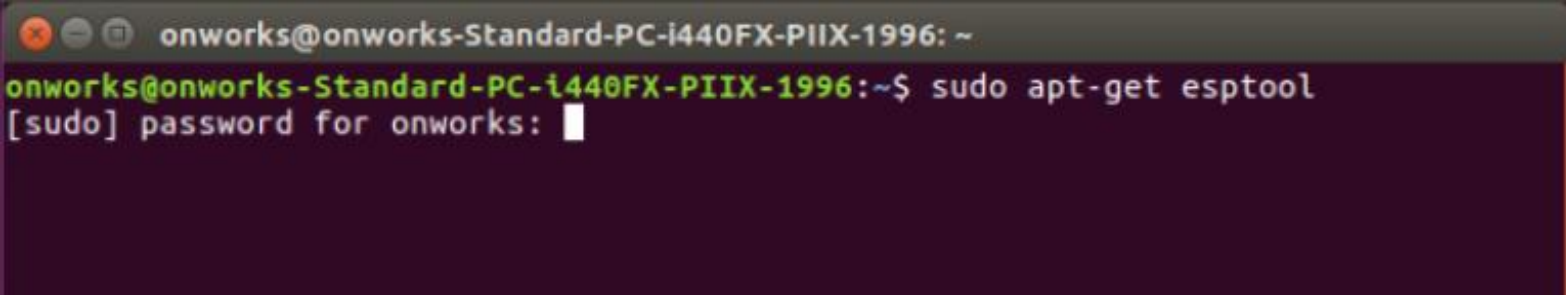
\includegraphics[width=1\textwidth]{figures/apt_get_esptool.png}
    \caption{Installing esptool package on Ubuntu.}
\end{figure}

Next you need to install python, if you don't have it, since the esptool is written in python language. So
you need to type the command \textit{“sudo apt-get python”}, as shown in the image. Again, if
prompted, type in the password of the sudo user, then press ENTER and wait.

\begin{figure}[H]
    \centering
    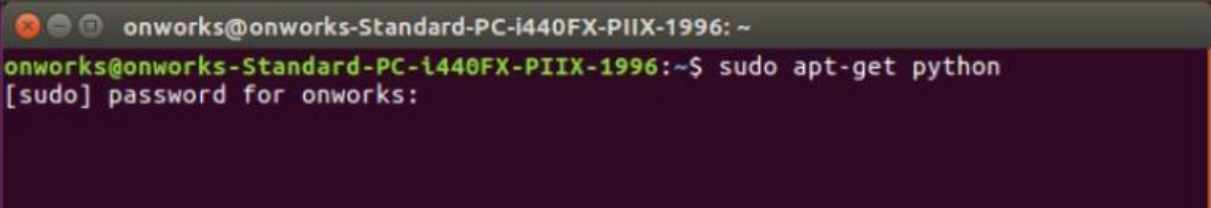
\includegraphics[width=1\textwidth]{figures/apt_get_python.png}
    \caption{Installing python package on Ubuntu.}
\end{figure}

Once we have installed both packages type \textit{“sudo tail -f /var/log/messages”} in the
terminal as shown in the image to monitor in real-time the log file, that will show us
which COM the black box will be associated to by the OS. If prompted, type in the
password of the sudo user, then press ENTER. \textbf{Now we can plug in the black box}.

\begin{figure}[H]
    \centering
    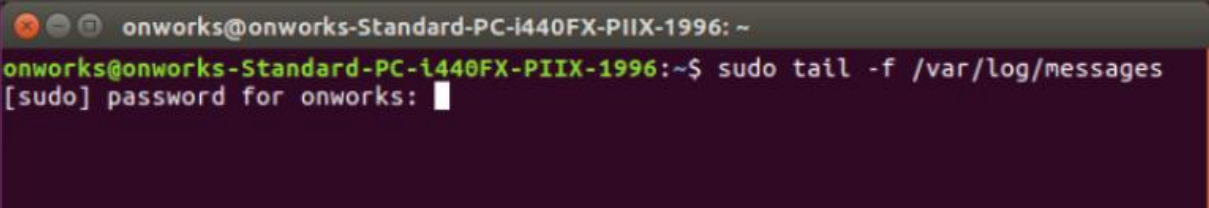
\includegraphics[width=1\textwidth]{figures/tail_com.png}
    \caption{Monitor real-time COM connections.}
\end{figure}

The black box has a small microUSB connector on the rear side, as you can see in 
Figure~\ref{fig:black_box_labels}. So, connect the microUSB cable side and to the
black box. After that, connect the USB side of the cable to a free USB port on your computer.

\textbf{REMEMBER!} Both sides of the cable fits only in one way in the corresponding plugs, so
don't force them or you will risk to brake the ToM+ port or your computer one. Try turning it
to the other side and check if it works that way.\\

As soon as you plug the black box to the computer you should get an output similar
to this one shown in the block of code down here.

\begin{lstlisting}[language=bash]
Oct 15 11:05:14 Kubuntu2004 kernel: [ 172.232228] usb 1-3: new full-speed USB
device number 3 using xhci_hcd
Oct 15 11:05:14 Kubuntu2004 kernel: [ 172.423441] usb 1-3: New USB device found,
idVendor=10c4, idProduct=ea60, bcdDevice= 1.00
Oct 15 11:05:14 Kubuntu2004 kernel: [ 172.423453] usb 1-3: New USB device
strings: Mfr=1, Product=2, SerialNumber=3
Oct 15 11:05:14 Kubuntu2004 kernel: [ 172.423457] usb 1-3: Product: CP2102 USB
to UART Bridge Controller
Oct 15 11:05:14 Kubuntu2004 kernel: [ 172.423461] usb 1-3: Manufacturer: Silicon
Labs
85
Oct 15 11:05:14 Kubuntu2004 kernel: [ 172.423464] usb 1-3: SerialNumber: 0001
Oct 15 11:05:14 Kubuntu2004 mtp-probe: checking bus 1, device 3:
"/sys/devices/pci0000:00/0000:00:08.1/0000:03:00.3/usb1/1-3"
Oct 15 11:05:14 Kubuntu2004 mtp-probe: bus: 1, device: 3 was not an MTP device
Oct 15 11:05:14 Kubuntu2004 kernel: [ 172.457397] usbcore: registered new
interface driver usbserial_generic
Oct 15 11:05:14 Kubuntu2004 kernel: [ 172.457415] usbserial: USB Serial support
registered for generic
Oct 15 11:05:14 Kubuntu2004 kernel: [ 172.460166] usbcore: registered new
interface driver cp210x
Oct 15 11:05:14 Kubuntu2004 kernel: [ 172.460185] usbserial: USB Serial support
registered for cp210x
Oct 15 11:05:14 Kubuntu2004 kernel: [ 172.460236] cp210x 1-3:1.0: cp210x
converter detected
Oct 15 11:05:14 Kubuntu2004 kernel: [ 172.464538] usb 1-3: cp210x converter now
attached to ttyUSB0
Oct 15 11:05:14 Kubuntu2004 mtp-probe: checking bus 1, device 3:
"/sys/devices/pci0000:00/0000:00:08.1/0000:03:00.3/usb1/1-3"
Oct 15 11:05:14 Kubuntu2004 mtp-probe: bus: 1, device: 3 was not an MTP device
\end{lstlisting}

The line we are interested in is this one: \textit{“cp210x converter now
attached to ttyUSB0”} where the word \textbf{“ttyUSB0”} is the serial
port where the black box is attached. So, note down this port, that can be different
from mine, because we will need it while uploading the new firmware.

\subsection{The updating workflow}

Navigate with your file manager in the folder where the firmware \textit{.bin} file is stored and
open a terminal in it by right clicking on the folder and selecting \textbf{“Open Terminal”}
option from the dropdown menu. Or if you prefer, you can manually navigate through
your folders using the “cd” command until you find the right one.

Once you are in the correct directory, execute this long and boring command, replacing \textit{“ttyUSBx”} with the
serial port name we noted down in the step before (e.g. \textit{“ttyUSB0”}) and \textit{“ESP32\textunderscore FwXX.bin”} with
the name of the \textit{“.bin”} file which contains the firmware version to load on ToM+
(e.g. \textit{“ESP32\textunderscore Fw23.bin”}).

\begin{verbatim}
    python /usr/share/esptool/esptool.py --chip auto --port /dev/ttyUSBx --baud
921600 --before default_reset --after hard_reset write_flash -z --flash_mode dio
--flash_freq 40m --flash_size 4MB 0x10000 ESP32_FwXX.bin
\end{verbatim}

You should receive an output similar to the following one:

\begin{lstlisting}[language=bash]
Serial port /dev/ttyUSB0
Connecting........_____.....____
Detecting chip type... ESP32
Chip is ESP32D0WDQ5 (revision 3)
Features: WiFi, BT, Dual Core, 240MHz, VRef calibration in efuse, Coding Scheme
None
Crystal is 40MHz
MAC: xx:xx:xx:xx:xx:xx
Changing baud rate to 921600
Changed.
Enabling default SPI flash mode...
Configuring flash size...
Erasing flash...
Compressed 716176 bytes to 461048...
Took 2.90s to erase flash block
Wrote 716176 bytes (461048 compressed) at 0x00010000 in 9.1 seconds (effective
630.3 kbit/s)...
Hash of data verified.
Leaving...
Hard resetting via RTS pin...
\end{lstlisting}

Now close this window and all the others and then you can safely unplug the cable
from both your PC and ToM+. Only after this actions, you can restore the normal power supply of ToM+,
moving the switch to the 1 state and powering on your Twizy using the ignition key.

To restore your previous configurations, enter in the ToM+ settings page by pressing
the three dots in the top right corner and then press the exit button without doing
anything. Doing that way you will update the data structure saved in black box
memory and your configurations are back too.\\

\textbf{Congratulations!} You've finished the whole updating process, now enjoy the new firmware
and remember to report any bugs or problems to me through private messages, attaching 
an image perhaps.